\subsection{Top-Level Overview Diagram of the alamSYS and Its Interactions to External Systems}
\label{subsec:top_level_overview}

% Sytem Overview Diagram
\begin{figure}[ht]
    \centering
    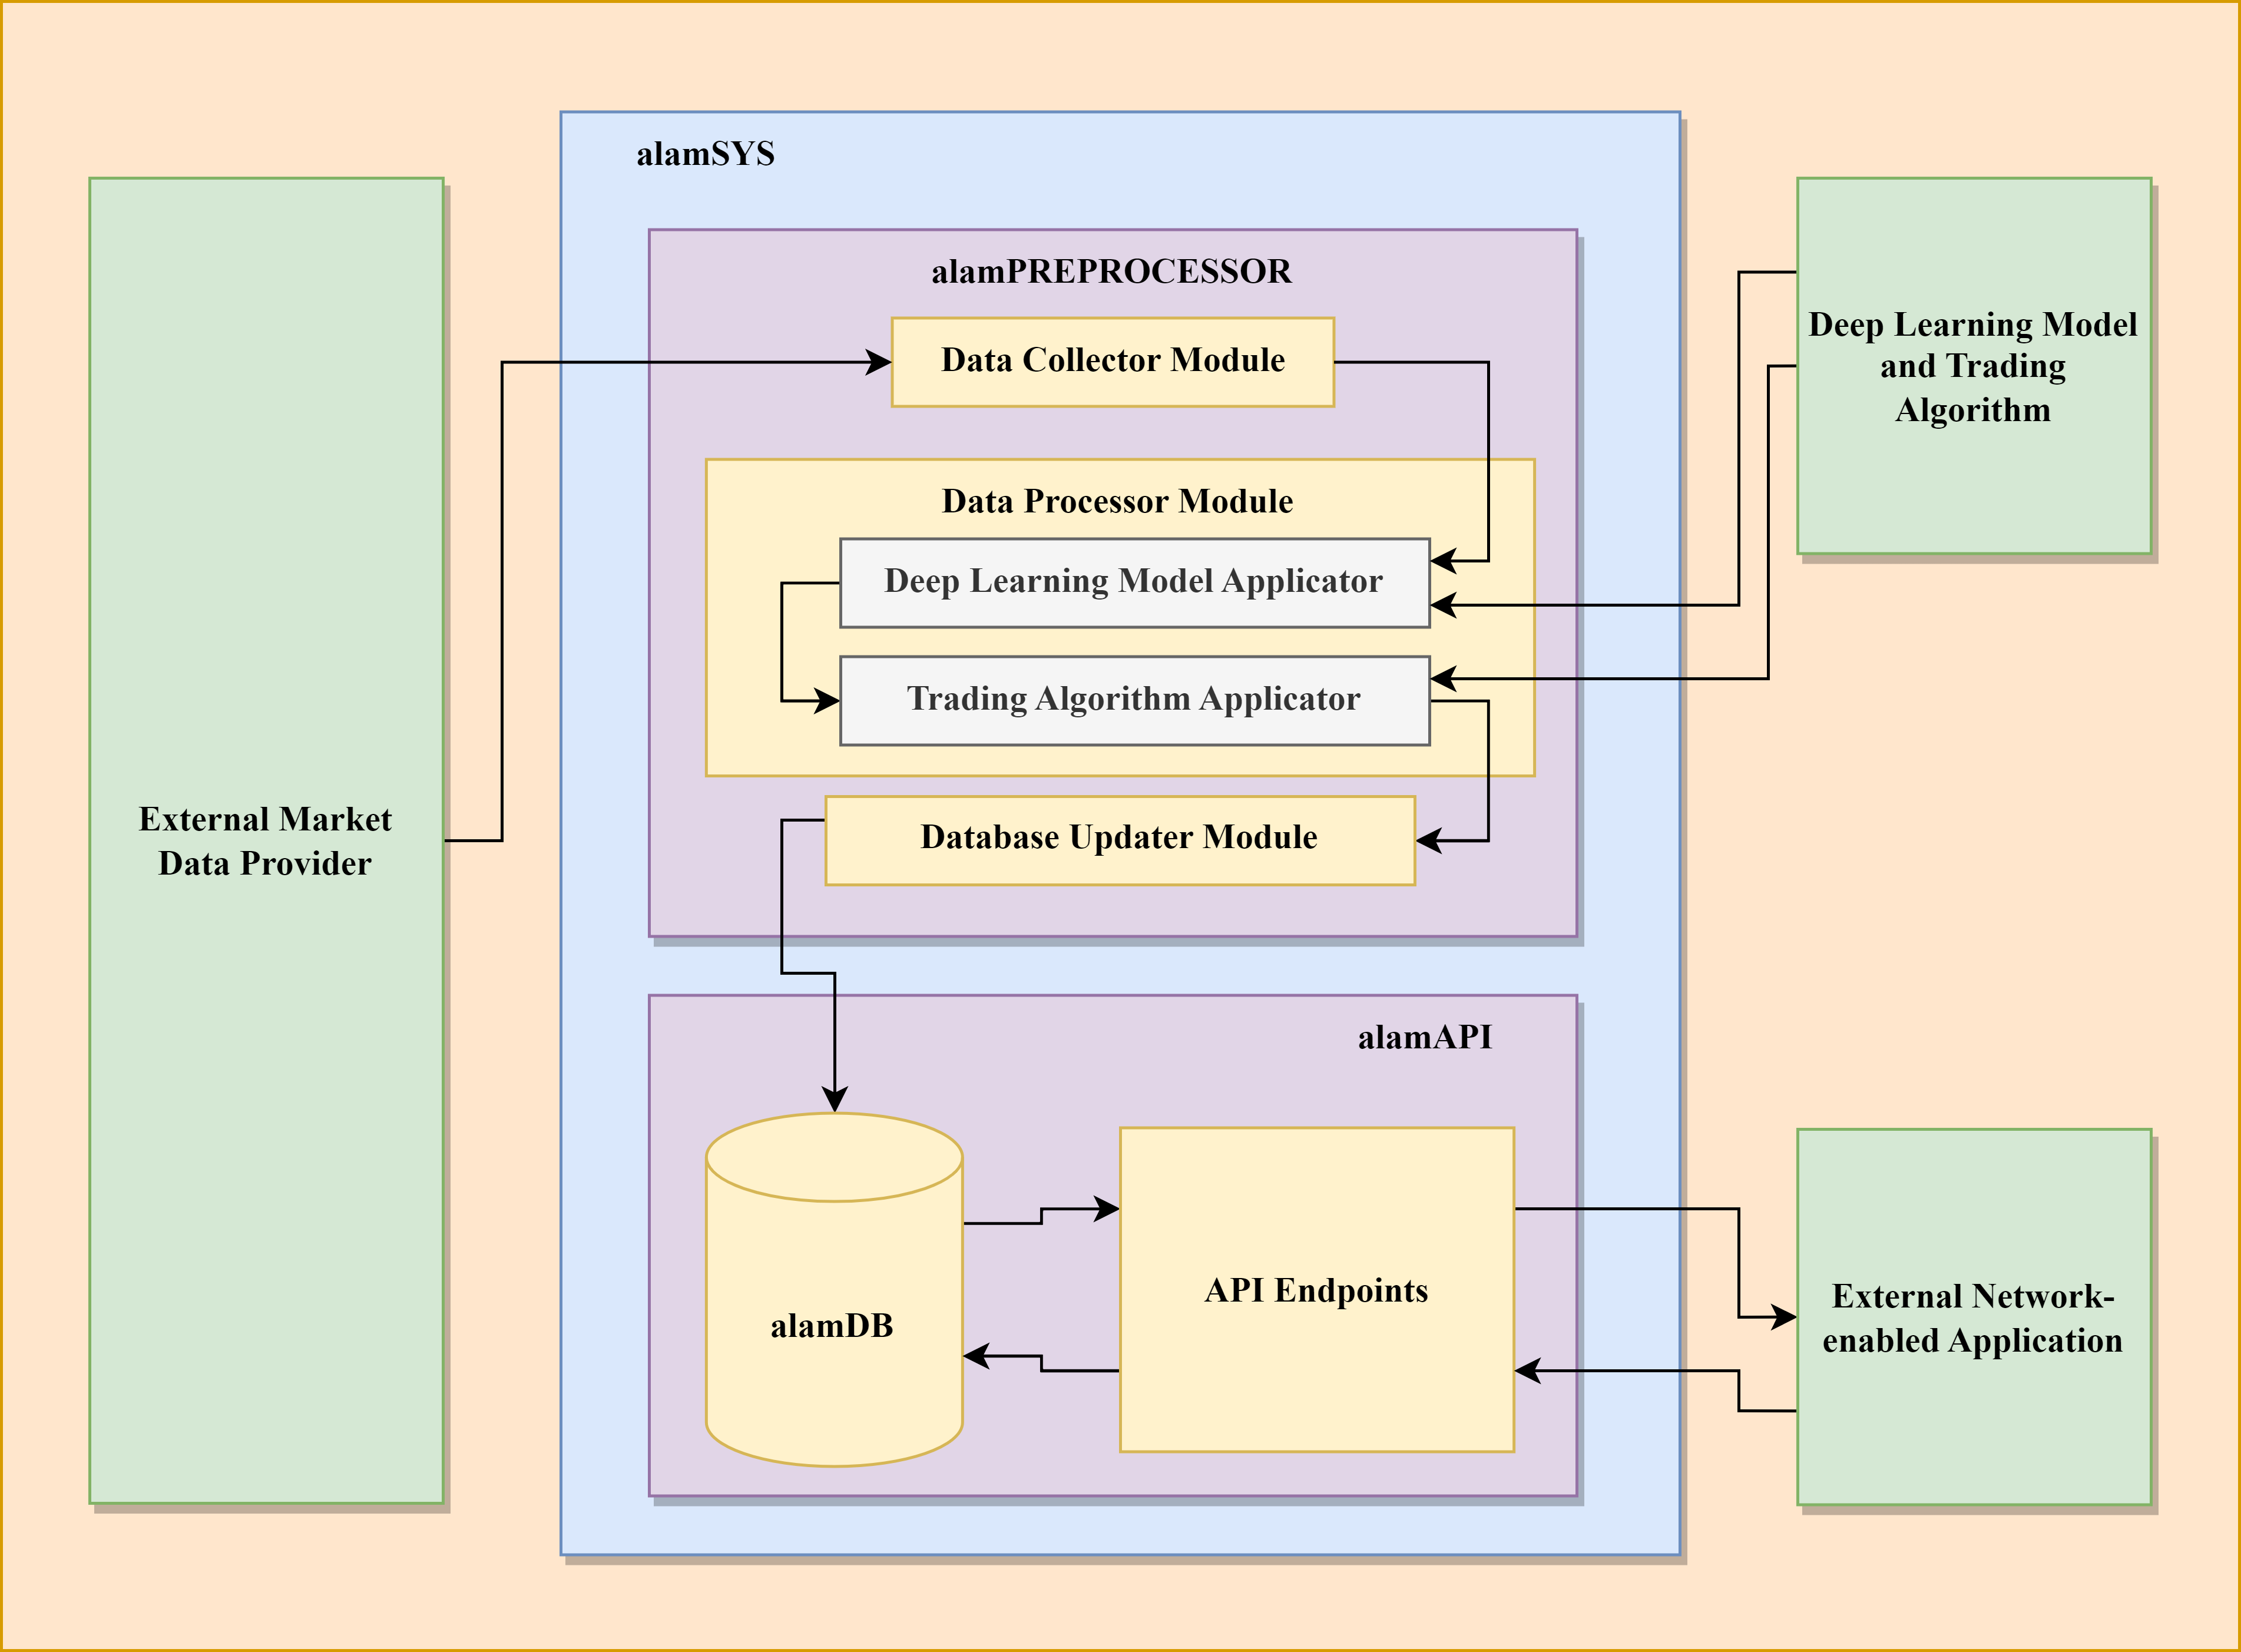
\includegraphics[height=0.45\textheight]{./assets/Chapter_3/SystemOverview.png}
    \caption{Top-Level Overview of the alamSYS and Interactions with External Applications/Systems}
    \label{fig:system_overview}
\end{figure}
\FloatBarrier

Figure \ref{fig:system_overview} shows the top-level overview of the 
alamSYS and its interactions to any third-party or external applications. 
The alamSYS is connected to three external 
entities: (1) External Market Data Provider, which provides the system with the 
needed historical market data; (2) Deep Learning Model and Trading Algorithm, 
in the case of this special problem, a deep learning model was developed and 
utilized by the system, however as previously discussed the system is 
created to accept any other machine learning models and or proprietary trading algorithms 
that other developers may or want to develop in the future; and 
(3) External Application, which can be a web-based or mobile-based application, that
utilizes the functionalities provided by the alamSYS, through the
API endpoints.
\hfill \\

On the middle of the diagram the alamSYS is observed to have three main components, 
namely, (1) alamPREPROCESSOR, which is further divided into sub-components: 
(a) Data Collector Module (DCM), which collects the data from the external market data provider; 
(b) Data Processor Module (DPM), which processes the historical market data collected by 
applying the developed machine learning model and sending it to the (c) Database Updater
Module (DUM); (2) alamDB, which is based on MongoDB, which is a document-based and non-relational 
database; finally, the database is connected to the (3) alamAPI, which contains the 
API endpoints which processes the request and responses of the system to any external 
application connected to the API via a network.